\section*{Results}
\label{Results}
%
The probability of choosing one stimuli over another is calculated for each comparison as explained in \autoref{eq:probability}. The results for the probabilities are shown in \autoref{tab:prob}. 
%
\begin{table}[H]
\centering
\begin{tabular}{@{}llllllll@{}}
\toprule
Drugs      & No. & 1    & 2    & 3    & 4    & 5    & 6    \\ \midrule
Alcohol    & 1   & 0    & 0.58 & 0.73 & 0.21 & 0.08 & 0.15 \\
Tobacco    & 2   & 0.42 & 0    & 0.38 & 0.04 & 0    & 0.06 \\
Cannabis   & 3   & 0.27 & 0.63 & 0    & 0.06 & 0.02 & 0    \\
Ecstasy    & 4   & 0.79 & 0.96 & 0.94 & 0    & 0.02 & 0.35 \\
Heroin     & 5   & 0.91 & 1    & 0.98 & 0.98 & 0    & 0.92 \\
Cocaine    & 6   & 0.85 & 0.94 & 1    & 0.65 & 0.83 & 0    \\ \bottomrule
\end{tabular}
\caption{The probability that one stimulus is chosen over another stimulus.}
\label{tab:prob}
\end{table} 
\noindent 
%
To find out how many times the stochastic transitivities is violated, each of the three types is investigated and the number of times there is a violation is counted. The results are shown in \autoref{tab:Stocha}. 
%
\begin{table}[H]
\centering
\begin{tabular}{@{}ll@{}}
\toprule
Stochastic transitivity     & Violations \\ \midrule
WST      & 0   \\
MST      & 1   \\
SST      & 5   \\ \bottomrule
\end{tabular}
\caption{Results for the number of violations of the three stochastic transitivities out of 20 possible.}
\label{tab:Stocha}
\end{table}

\subsection*{BTL-model}
To check how good a fit the BTL-model is, a Chi-square test is conducted and the results are shown in \autoref{tab:Chi}. 
%
\begin{table}[H]
\centering
\begin{tabular}{@{}lll@{}}
\toprule
$\chi^{2}$   & Df  & p-value \\ \midrule
24.9423      & 10  & 0.0055* \\ \bottomrule
\end{tabular}
\caption{Results from the Chi-square test. The p-value of 0.0055 suggests that the BTL model does not fit.}
\label{tab:Chi}
\end{table} 
\noindent 
The results from the Chi-square test shows a p-value at 0.0055 and therefore the conclusion is that this model is significant worse at predicting the data than the statistic model. The model is not accepted and instead the Preference Tree will be used. 

\subsection*{Preference Tree}
The way it is determined how the Preference Tree should be structured is be drawing the tree be looking at the types of drugs and conducting a Chi-square on the model to see if it fits. Many different Preference Trees were drawn and tested, the first one found that fits is shown in \autoref{fig:Tree1overveiw}
%
\begin{figure}[H]
\centering
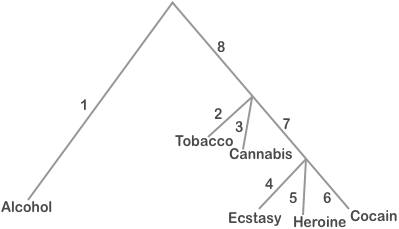
\includegraphics[width = 0.70\textwidth]{Figure/Tree1overview}
\caption{Structure of the first Preference Tree found that fits the data.}
\label{fig:Tree1overveiw}
\end{figure}
\noindent
%
The results of the Chi-square test for the Preference Tree shown at \autoref{fig:Tree1overveiw} are shown in \autoref{tab:Chi}. 
%
\begin{table}[H]
\centering
\begin{tabular}{@{}lll@{}}
\toprule
$\chi^{2}$   & Df  & p-value \\ \midrule
12.7157      & 8   & 0.1220  \\ \bottomrule
\end{tabular}
\caption{Results from the Chi-square test on the first Preference Tree. The p-value of 0.1220 suggests that the Preference model fits.}
\label{tab:Chi1}
\end{table} 
\noindent
%
One other preference tree was found to fit, and this tree is shown in \autoref{fig:Tree2overveiw}. 
%
\begin{figure}[H]
\centering
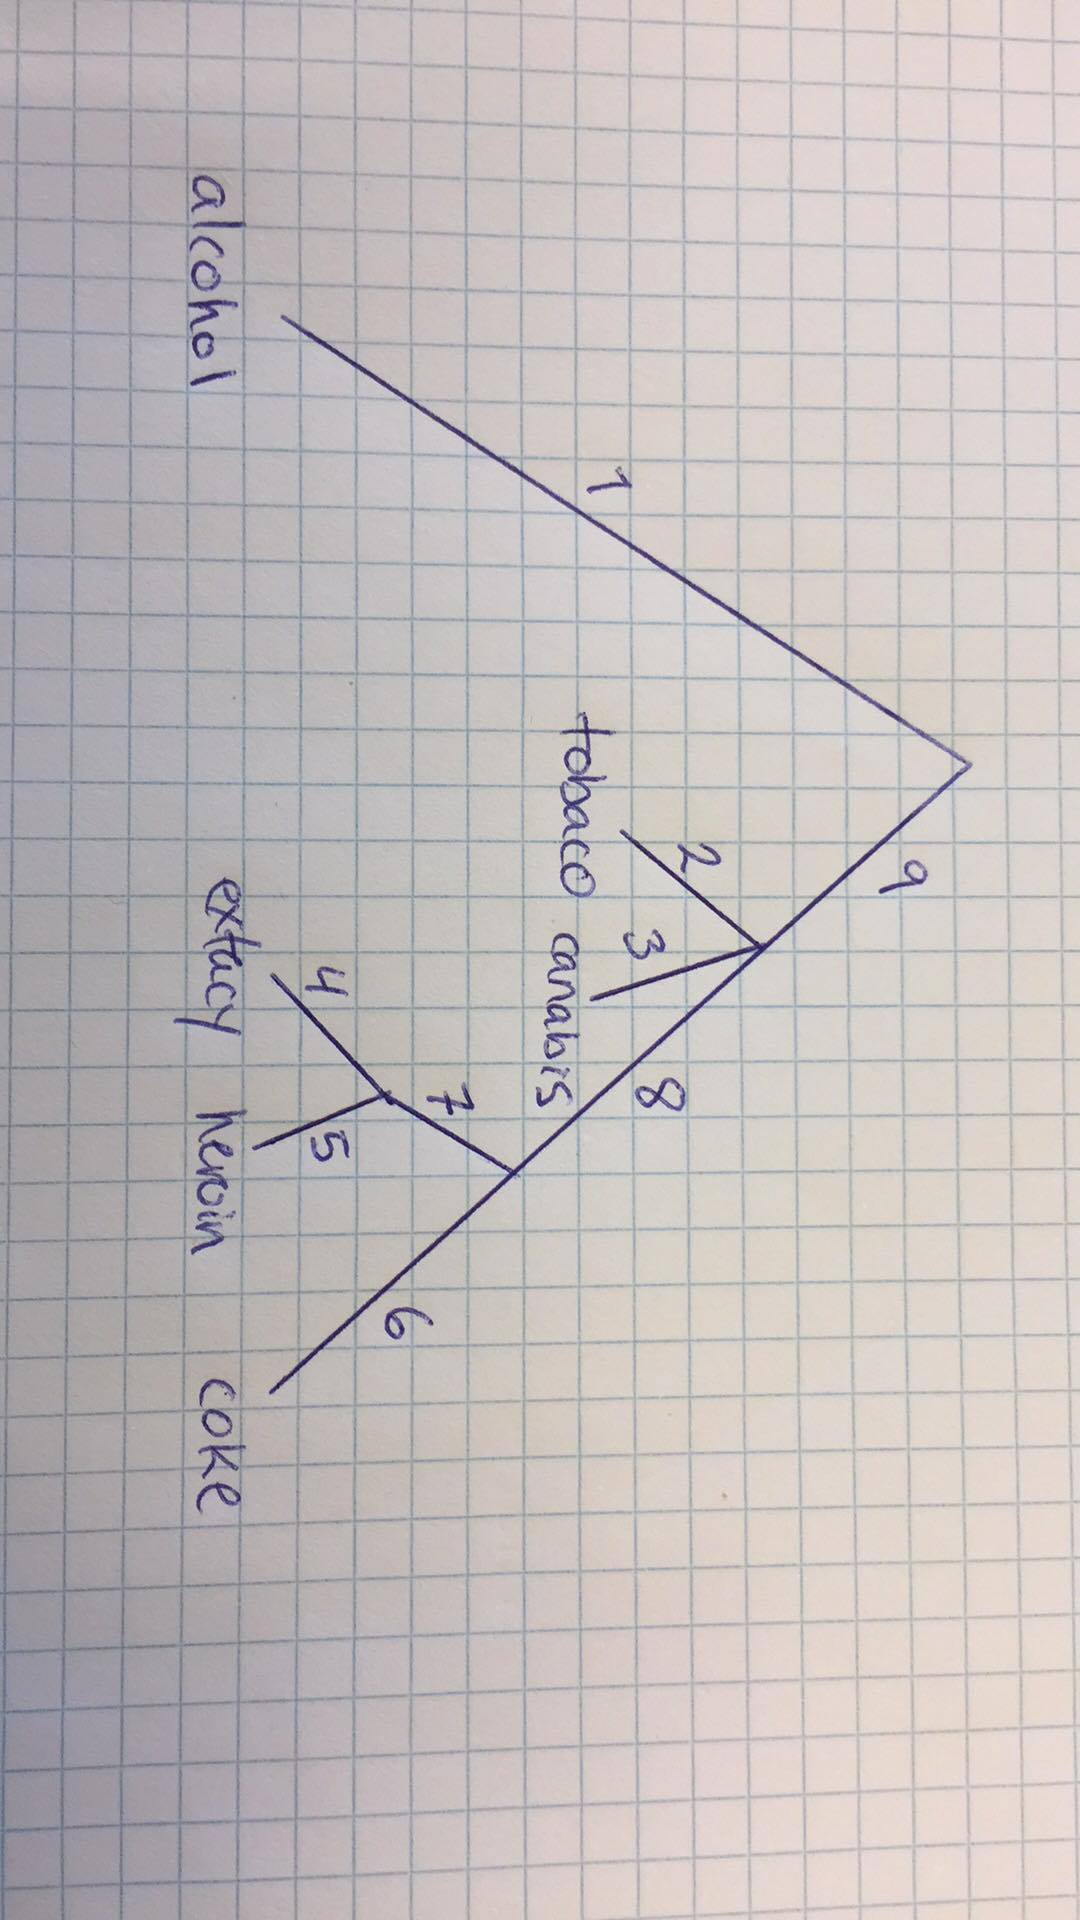
\includegraphics[width = 0.70\textwidth]{Figure/Tree2overview}
\caption{Structure of the second Preference Tree found that fits the data.}
\label{fig:Tree2overveiw}
\end{figure}
\noindent
%
The results of the Chi-square test for the second Preference Tree shown at \autoref{fig:Tree2overveiw} are shown in \autoref{tab:Chi2}. 
%
\begin{table}[H]
\centering
\begin{tabular}{@{}lll@{}}
\toprule
$\chi^{2}$   & Df  & p-value \\ \midrule
10.9377      & 7   & 0.1414  \\ \bottomrule
\end{tabular}
\caption{Results from the Chi-square test on the second Preference Tree. The p-value of 0.1220 suggests that the Preference model fits.}
\label{tab:Chi2}
\end{table} 